\section{Аннотация}\label{ux430ux43dux43dux43eux442ux430ux446ux438ux44f}

Краткосрочное прогнозирование электрической нагрузки является ключевым
компонентом эксплуатации интеллектуальных энергосетей, опережающего
планирования и промышленного энергоменеджмента. В работе представлен
воспроизводимый бенчмарк, сравнивающий два классических базовых метода
(SeasonalNaive и грид-настроенный SARIMA), модель градиентного бустинга
(XGBoost), три нейросетевые архитектуры (DLinear, PatchTST,
iTransformer) и две фундаментальные модели временных рядов
(Chronos-Bolt-Small и TimesFM 2.5). Основная оценка проводится на наборе
ECL по агрегированной нагрузке. ETTh1 используется как вторичный
промышленный бенчмарк с целевой переменной HUFL --- load-related
transformer variable; температура масла OT целенаправленно не
рассматривается как электрическая нагрузка. Эксперименты охватывают
горизонты 24, 96 и 168 часов при фиксированном контексте 336 часов. На
ECL три лидирующие модели --- TimesFM, Chronos-Bolt и XGBoost ---
отличаются друг от друга в пределах примерно 0.1--0.4 \% по горизонтам:
TimesFM незначительно лучше при H=24, XGBoost --- при H=96 и H=168;
грид-настроенный SARIMA закрывает большую часть оставшегося разрыва без
обучаемых признаков. На ETTh1/HUFL Chronos-Bolt лучшая при H=24, DLinear
--- при H=96 и H=168. Результаты показывают, что фундаментальные модели
конкурентоспособны в zero-shot режиме, но классические и обучаемые на
целевом ряду модели остаются сильными при наличии данных и инженерии
признаков.

\textbf{Ключевые слова:} краткосрочное прогнозирование нагрузки;
временные ряды; глубокое обучение; фундаментальные модели; SARIMA;
XGBoost; интеллектуальная сеть.

\section{1. Введение}\label{ux432ux432ux435ux434ux435ux43dux438ux435}

Краткосрочное прогнозирование нагрузки (STLF) поддерживает диспетчерское
планирование, балансировку, тарифно-ориентированное управление,
планирование обслуживания и аномально-чувствительный промышленный
энергоменеджмент. В современных задачах smart-grid и Industry 4.0 от
моделей прогноза требуется не только точность, но и воспроизводимость,
вычислительная экономичность и устойчивость к различным режимам
эксплуатации.

Методологический ландшафт широк. Классические методы, такие как
ARIMA-семейство и сезонные наивные базовые модели, остаются важными
референсами; модели машинного обучения вроде градиентного бустинга
привлекательны тем, что включают лаговые и календарные признаки при
умеренной инженерии; современные модели глубокого обучения и
фундаментальные модели обещают более широкую переносимость между
доменами временных рядов. Это порождает практический вопрос: когда
дорогие архитектуры или zero-shot фундаментальные модели действительно
превосходят сильные недорогие базовые методы?

В работе представлено воспроизводимое исполнение бенчмарка на двух
открытых наборах данных. Прагматический вклад состоит в следующем:

\begin{itemize}
\tightlist
\item
  сквозной репозиторий с валидацией данных, leakage-aware шкалированием,
  метриками, измерением времени, фигурами и сборкой статьи;
\item
  реальные результаты для SeasonalNaive, грид-настроенного SARIMA,
  XGBoost, DLinear, PatchTST, iTransformer, Chronos-Bolt-Small и TimesFM
  2.5;
\item
  тесты Дибольда--Мариано, рассчитанные по поокно-ошибкам для топ-пар
  моделей;
\item
  анализ accuracy--latency, отделяющий стоимость развёртывания от чистой
  точности.
\end{itemize}

\begin{figure}
\centering
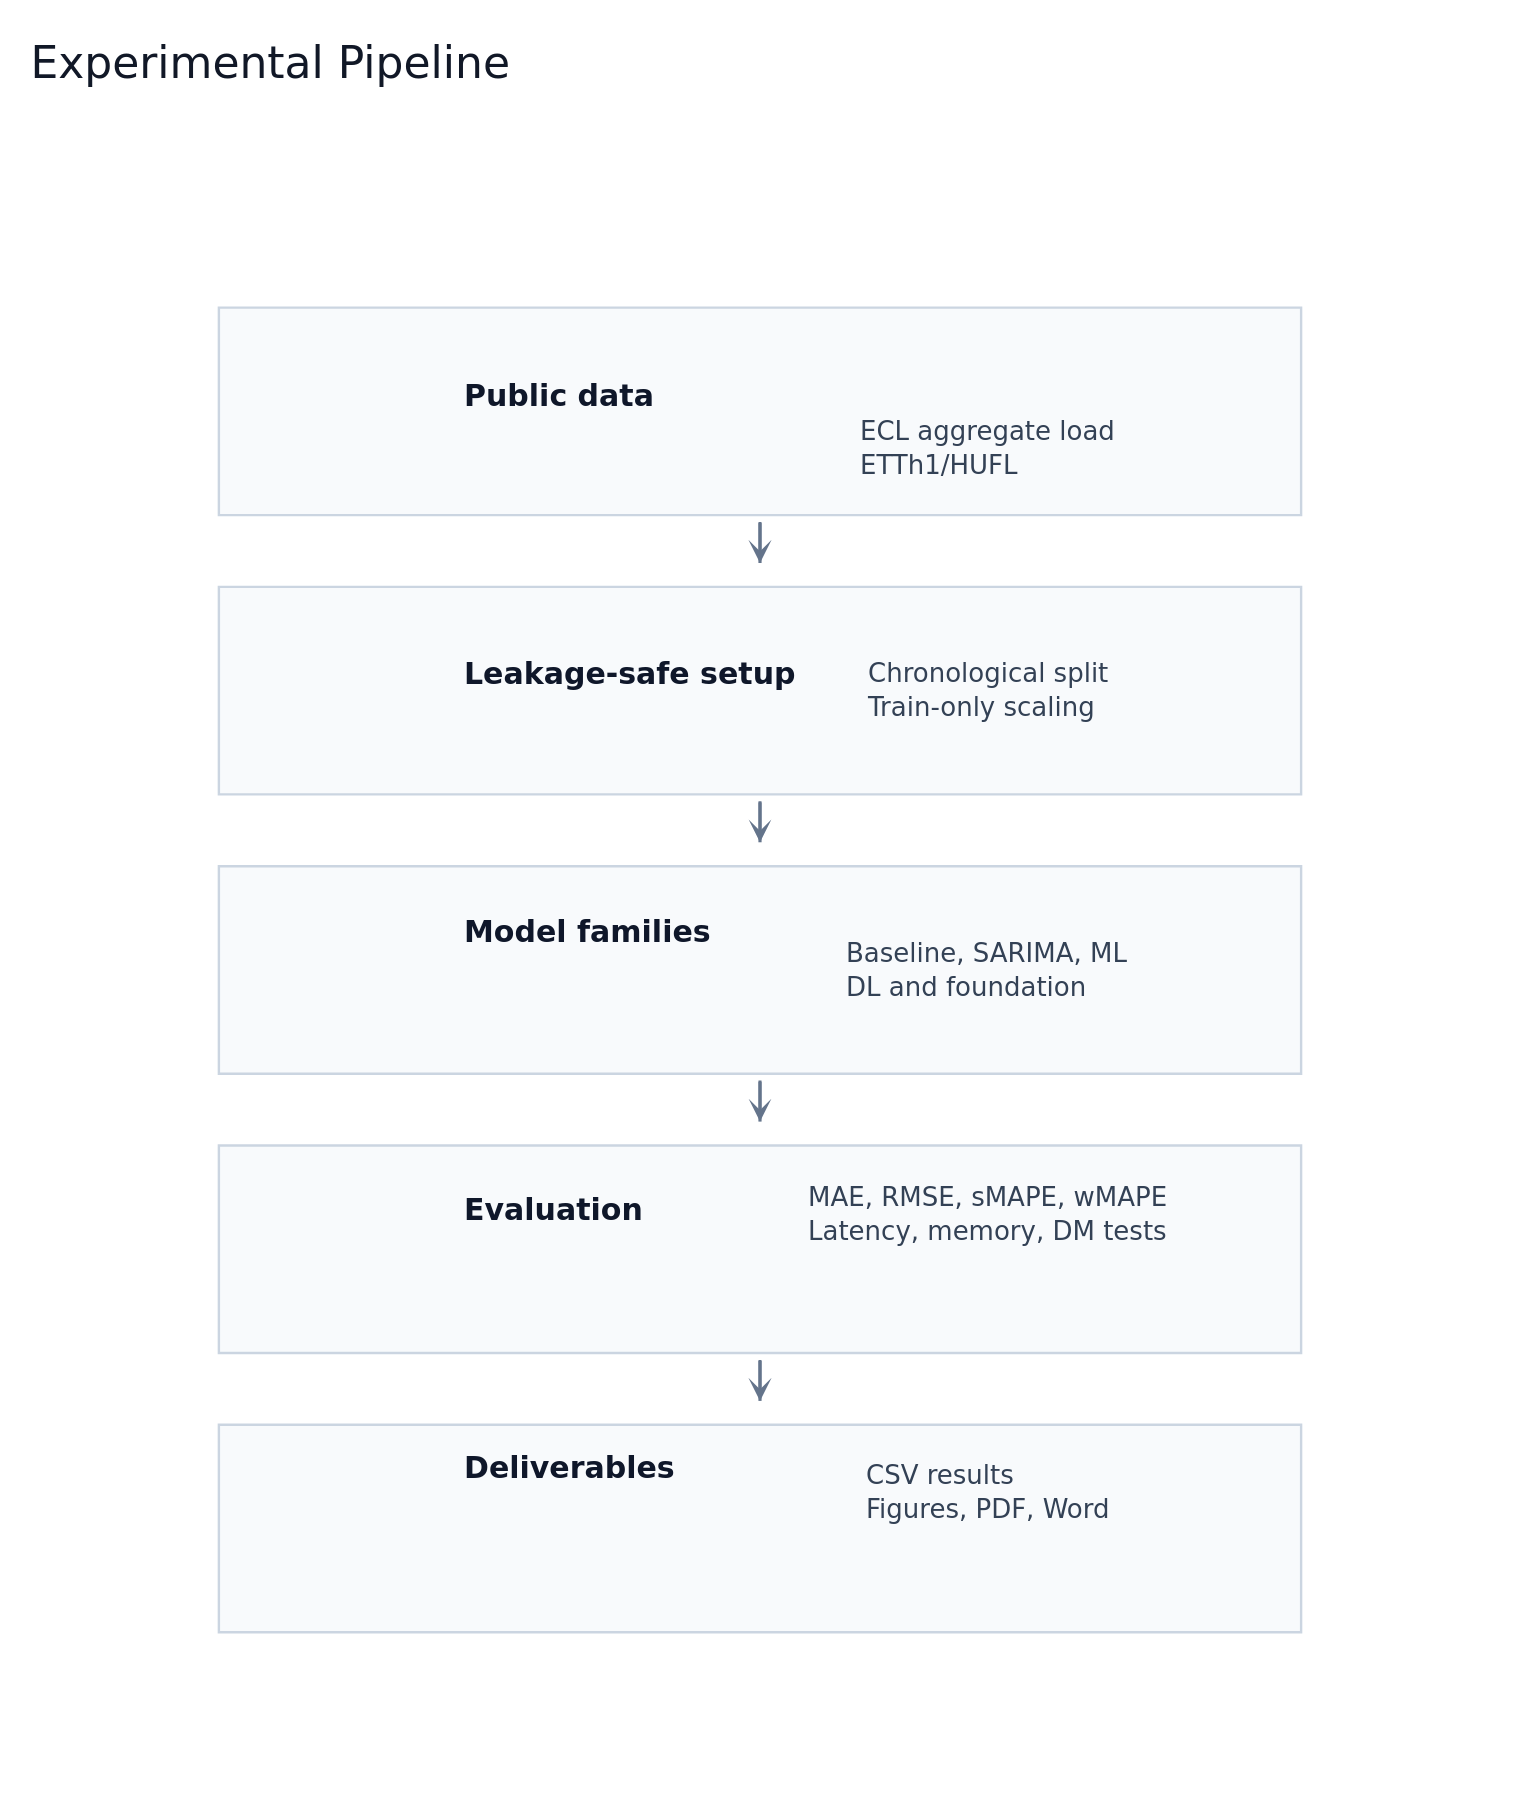
\includegraphics[width=6.6in,height=\textheight,keepaspectratio,alt={Рис. 1. Экспериментальный пайплайн.}]{docx_figures/fig1_methodology.png}
\caption{Рис. 1. Экспериментальный пайплайн.}
\end{figure}

\section{2. Обзор
литературы}\label{ux43eux431ux437ux43eux440-ux43bux438ux442ux435ux440ux430ux442ux443ux440ux44b}

Классические методы прогнозирования временных рядов, в частности
ARIMA-семейство, остаются важными, потому что задают интерпретируемые и
недорогие референсы; автоматический выбор порядков по информационным
критериям, таким как AICc, делает их применимыми по отдельным рядам
(Hyndman и Khandakar 2008 г.). Подходы машинного обучения на основе
лагов, календарных переменных и градиентно-бустированных деревьев широко
используются в задачах прогнозирования нагрузки благодаря быстрому
обучению и устойчивости при инженерии табличных признаков (Chen и
Guestrin 2016 г.).

Модели глубокого обучения, такие как LSTM (Hochreiter и Schmidhuber 1997
г.), архитектуры с механизмом внимания (Vaswani и др. 2017 г.), Informer
(Zhou и др. 2021 г.), DLinear (Zeng и др. 2023 г.), PatchTST (Nie и др.
2023 г.), iTransformer (Liu и др. 2024 г.), TimesNet (Wu и др. 2023 г.),
существенно расширили инструментарий долгосрочного прогнозирования.
Фундаментальные модели временных рядов, такие как TimesFM (Das и др.
2024 г.) и семейство Chronos (Ansari и др. 2024 г.), мотивируют новую
ось оценки: безобучаемое инференс-время против полноценного обучения на
целевом наборе.

Корректное сравнение должно учитывать риск того, что открытые бенчмарки
могли быть включены в претрейнинговые корпуса. Поэтому zero-shot
результаты на ECL или ETT нельзя интерпретировать как гарантированную
обобщающую способность на невиданных данных. Узкое и воспроизводимое
утверждение в этой работе: Chronos-Bolt и TimesFM запускались без
обучения на целевом наборе в рамках данного репозитория.

\section{3.
Методология}\label{ux43cux435ux442ux43eux434ux43eux43bux43eux433ux438ux44f}

При заданном одномерном контекстном окне задача состоит в предсказании
следующих H наблюдений для горизонтов H из множества \{24, 96, 168\}.
Эксперименты используют фиксированную длину контекста L = 336 часов, что
включает суточную и недельную сезонные компоненты и допускает
использование лага 168.

Базовая модель SeasonalNaive повторяет последний наблюдённый суточный
сезонный паттерн. Базовая модель SARIMA использует выбор порядков по
AICc на обучающей выборке из фиксированного грида, после чего выбранная
модель применяется к тестовым окнам через фильтрацию состояния, без
переподгонки на каждом окне. XGBoost обучается как прямой многошаговый
регрессор на лагах 1, 24, 168, скользящих средних по 24 и 168 часам и
циклических календарных признаках. DLinear, PatchTST и iTransformer
обучаются через NeuralForecast в той же одноцелевой постановке, с
коротким validation-only перебором learning-rate по 1e-3 и 5e-4 и ранним
остановом. Chronos-Bolt-Small и TimesFM 2.5 оцениваются в zero-shot
режиме без обучения на целевом ряду.

Все процедуры предобработки для обучаемых моделей подгоняются только на
тренировочной части, а метрики считаются после обратного преобразования
предсказаний на исходную шкалу целевой переменной. Фундаментальные
модели и SARIMA оцениваются непосредственно в исходной шкале.

\section{4. Постановка
эксперимента}\label{ux43fux43eux441ux442ux430ux43dux43eux432ux43aux430-ux44dux43aux441ux43fux435ux440ux438ux43cux435ux43dux442ux430}

Основной набор данных --- ECL, обработанный как агрегированная часовая
электрическая нагрузка по 321 клиенту. Вторичный набор --- ETTh1,
целевая переменная HUFL. Переменная OT в ETTh1 --- температура масла и
не рассматривается как электрическая нагрузка. ECL разбивается
хронологически 70 \% train, 10 \% validation, 20 \% test. ETTh1
использует стандартное хронологическое разбиение 12 / 4 / 4 месяца.

Точность измеряется метриками MAE, RMSE, sMAPE и wMAPE. Эффективность
измеряется временем обучения, single-window inference latency (batch
size 1), числом обучаемых параметров и пиковым потреблением GPU-памяти.
XGBoost, DLinear, PatchTST и iTransformer оцениваются по пяти сидам
(42--46) и приводятся как среднее ± СКО. SeasonalNaive, SARIMA,
Chronos-Bolt и TimesFM являются single-run детерминированными или
zero-shot оценками и приводятся без межсидовой дисперсии.

Тесты Дибольда--Мариано вычисляются по поокно-ошибкам для двух
топ-моделей по MAE при сиде 42 для каждой пары (датасет, горизонт).
Поскольку усреднение по окнам и плоский поточечный MAE взвешивают ошибки
по-разному, ранжирование по статистическим тестам может слегка
отличаться от ранжирования таблиц при близких моделях.

\section{5.
Результаты}\label{ux440ux435ux437ux443ux43bux44cux442ux430ux442ux44b}

\begin{figure}
\centering
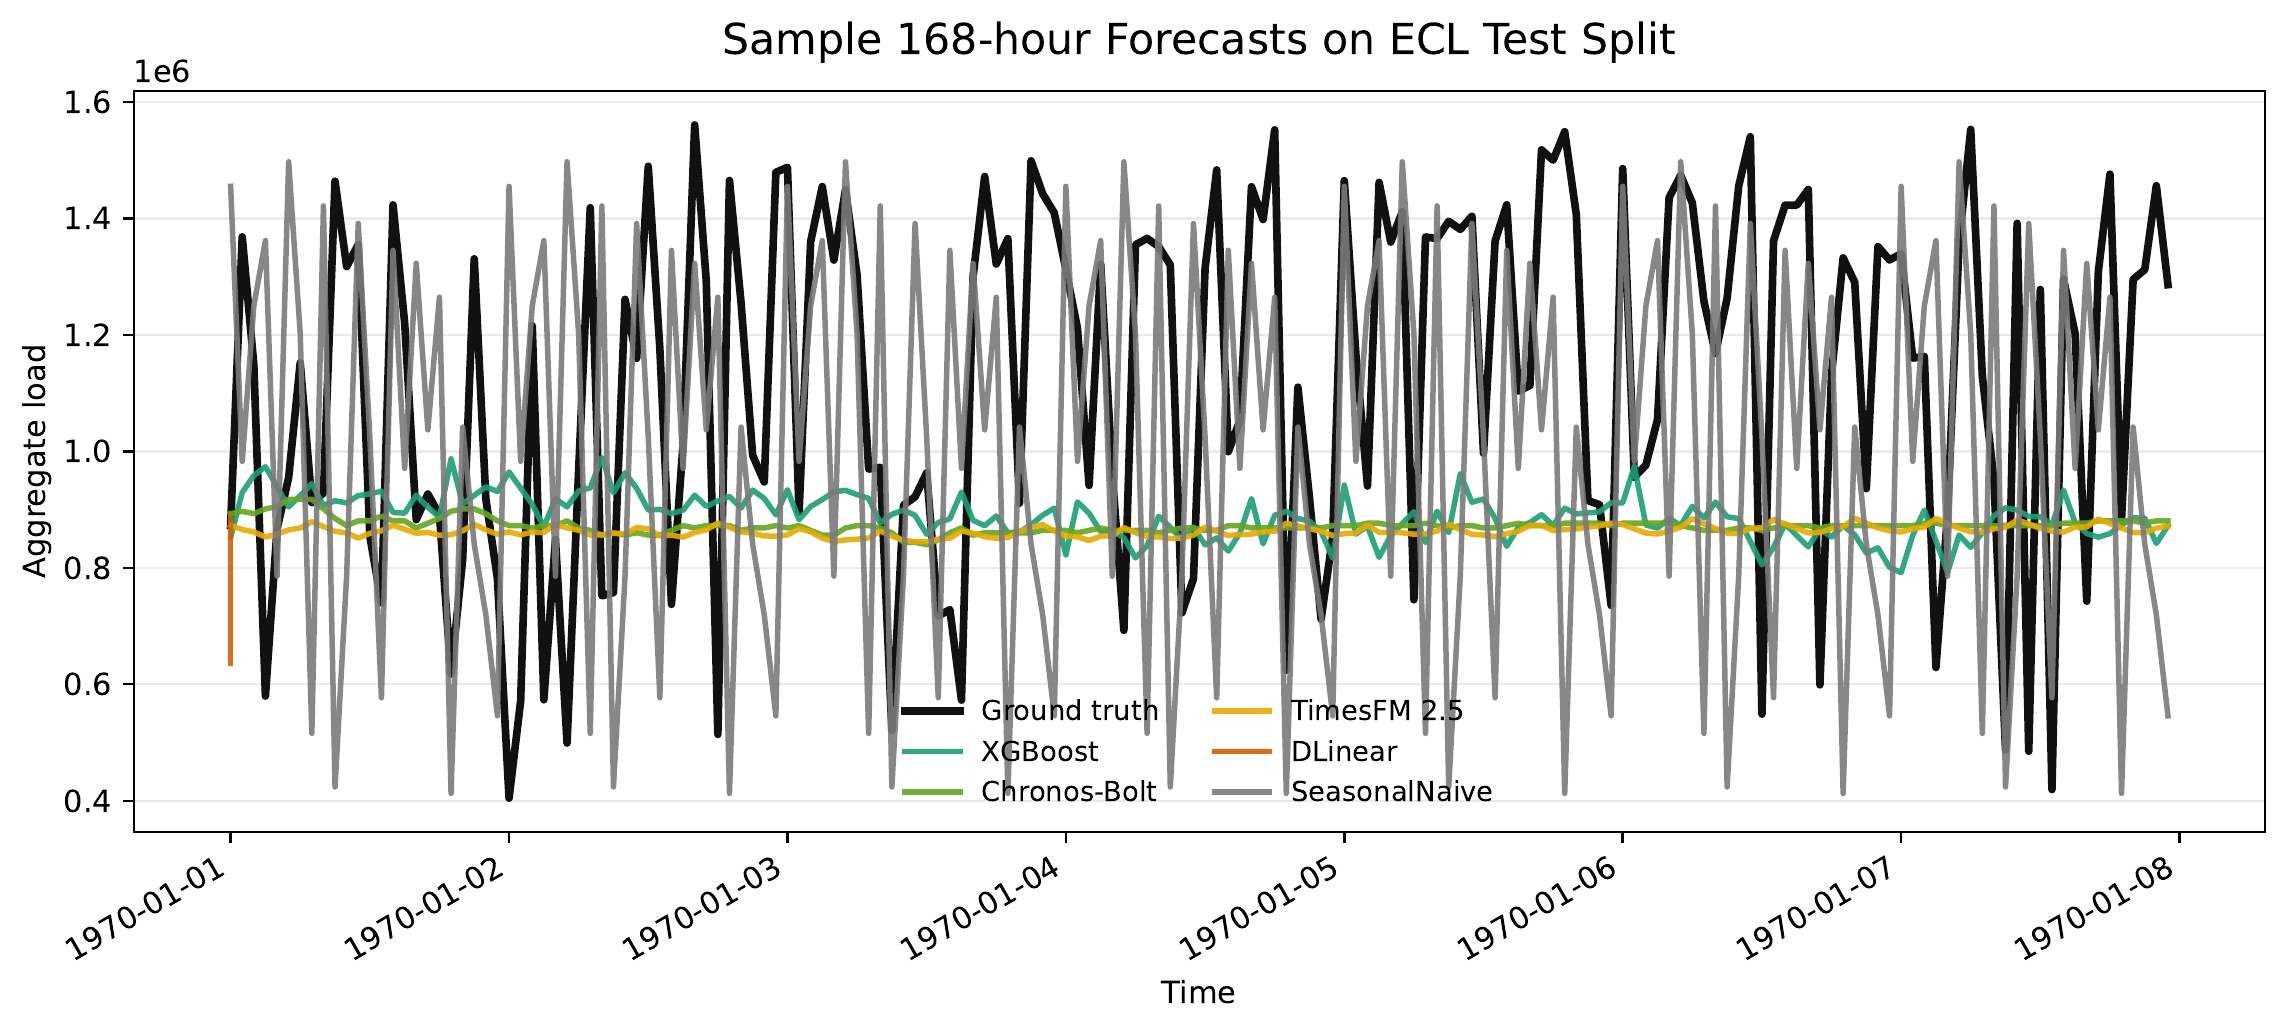
\includegraphics[width=6.6in,height=\textheight,keepaspectratio,alt={Рис. 2. Пример прогнозов на 168 часов для ECL у репрезентативных моделей.}]{docx_figures/fig2_forecasts.png}
\caption{Рис. 2. Пример прогнозов на 168 часов для ECL у
репрезентативных моделей.}
\end{figure}

\subsection{5.1 Точность на
ECL}\label{ux442ux43eux447ux43dux43eux441ux442ux44c-ux43dux430-ecl}

На ECL сильнейшую группу образуют XGBoost и две фундаментальные модели.
TimesFM имеет наименьший поточечный MAE при H=24, но разрыв до XGBoost и
Chronos-Bolt --- менее 0.1 \%, поэтому практическое ранжирование среди
этих трёх по сути плоское на коротком горизонте. На H=96 и H=168
незначительно лучше XGBoost, при этом Chronos-Bolt близок на всех трёх
горизонтах. Грид-настроенный SARIMA отстаёт от верхней группы на
небольшой, но устойчивый разрыв и опережает обучаемые нейросетевые
модели.

{\def\LTcaptype{none} % do not increment counter
\begin{longtable}[]{@{}
  >{\raggedright\arraybackslash}p{(\linewidth - 6\tabcolsep) * \real{0.2000}}
  >{\raggedleft\arraybackslash}p{(\linewidth - 6\tabcolsep) * \real{0.2667}}
  >{\raggedleft\arraybackslash}p{(\linewidth - 6\tabcolsep) * \real{0.2667}}
  >{\raggedleft\arraybackslash}p{(\linewidth - 6\tabcolsep) * \real{0.2667}}@{}}
\toprule\noalign{}
\begin{minipage}[b]{\linewidth}\raggedright
Модель
\end{minipage} & \begin{minipage}[b]{\linewidth}\raggedleft
H=24 MAE
\end{minipage} & \begin{minipage}[b]{\linewidth}\raggedleft
H=96 MAE
\end{minipage} & \begin{minipage}[b]{\linewidth}\raggedleft
H=168 MAE
\end{minipage} \\
\midrule\noalign{}
\endhead
\bottomrule\noalign{}
\endlastfoot
TimesFM 2.5 & \textbf{259345.28} & 262766.32 & 265044.60 \\
Chronos-Bolt & 259546.11 & 262601.94 & 264268.27 \\
XGBoost & 259549.38 ± 13.62 & \textbf{261792.58 ± 9.36} &
\textbf{264220.96 ± 24.77} \\
SARIMA & 263913.91 & 267033.48 & 271294.60 \\
DLinear & 278309.93 ± 78.45 & 279227.54 ± 52.48 & 280272.56 ± 47.26 \\
PatchTST & 279295.35 ± 274.56 & 280109.77 ± 94.31 & 280876.20 ±
109.22 \\
iTransformer & 283321.32 ± 278.79 & 279842.21 ± 148.37 & 279476.02 ±
103.81 \\
SeasonalNaive & 338935.90 & 340658.82 & 343510.17 \\
\end{longtable}
}

\begin{figure}
\centering
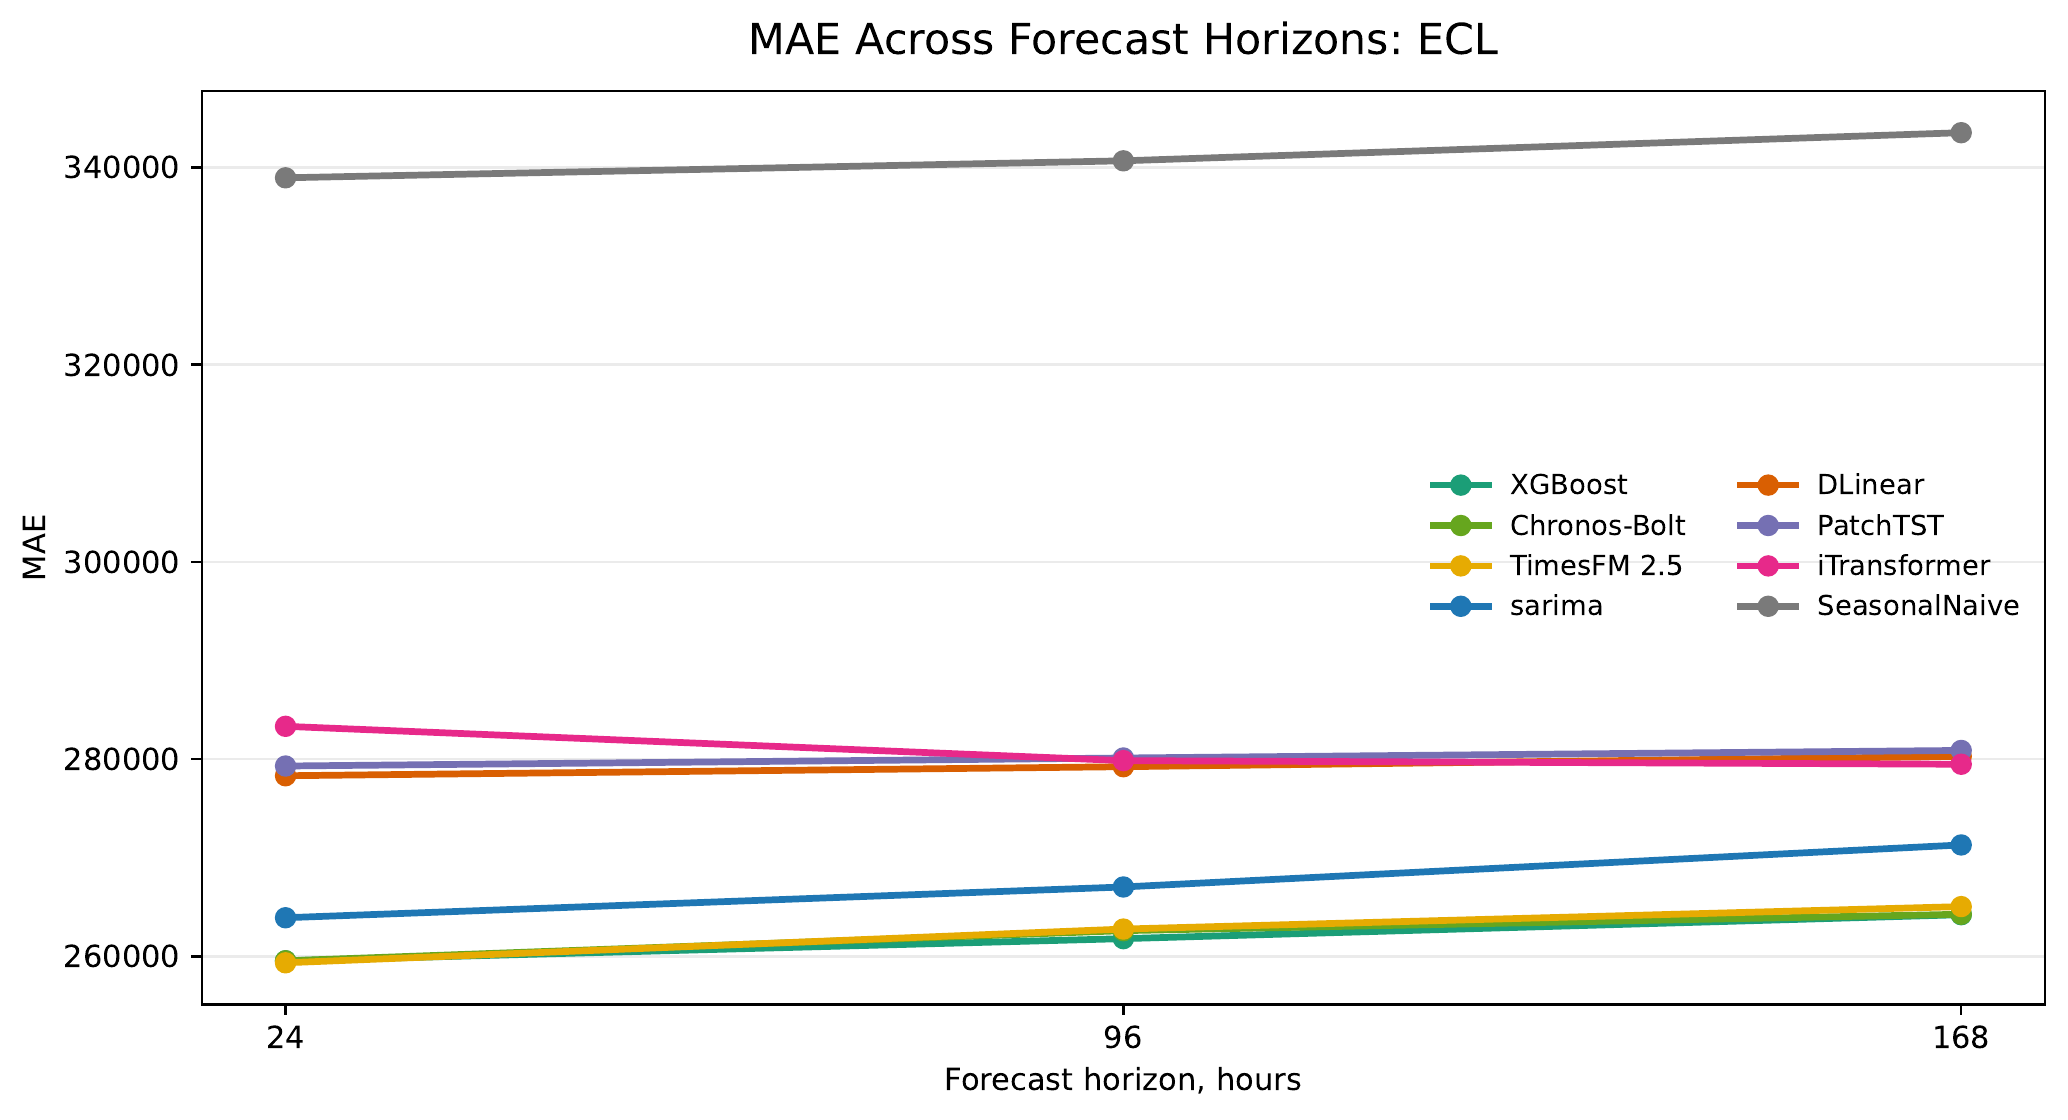
\includegraphics[width=6.6in,height=\textheight,keepaspectratio,alt={Рис. 3. MAE по горизонтам прогноза на ECL.}]{docx_figures/fig6_ecl_accuracy.png}
\caption{Рис. 3. MAE по горизонтам прогноза на ECL.}
\end{figure}

\subsection{5.2 Точность на
ETTh1/HUFL}\label{ux442ux43eux447ux43dux43eux441ux442ux44c-ux43dux430-etth1hufl}

На ETTh1/HUFL Chronos-Bolt лучшая при H=24. PatchTST --- сильнейшая
обучаемая модель на том же горизонте, DLinear лидирует при H=96 и H=168.
TimesFM конкурентен, но не лучший на этом бенчмарке. SARIMA близок к
лучшему классическому базовому методу и опережает XGBoost на всех трёх
горизонтах --- обратная ситуация по сравнению с ECL, где XGBoost
доминирует над SARIMA.

{\def\LTcaptype{none} % do not increment counter
\begin{longtable}[]{@{}lrrr@{}}
\toprule\noalign{}
Модель & H=24 MAE & H=96 MAE & H=168 MAE \\
\midrule\noalign{}
\endhead
\bottomrule\noalign{}
\endlastfoot
Chronos-Bolt & \textbf{3.00} & 3.57 & 3.77 \\
PatchTST & 3.04 ± 0.01 & 3.62 ± 0.03 & 3.95 ± 0.07 \\
DLinear & 3.08 ± 0.00 & \textbf{3.55 ± 0.00} & \textbf{3.70 ± 0.00} \\
TimesFM 2.5 & 3.16 & 3.67 & 3.79 \\
iTransformer & 3.25 ± 0.02 & 3.72 ± 0.01 & 3.91 ± 0.02 \\
SeasonalNaive & 3.31 & 3.92 & 4.18 \\
SARIMA & 3.45 & 3.90 & 4.18 \\
XGBoost & 3.89 ± 0.01 & 4.21 ± 0.01 & 4.27 ± 0.01 \\
\end{longtable}
}

\begin{figure}
\centering
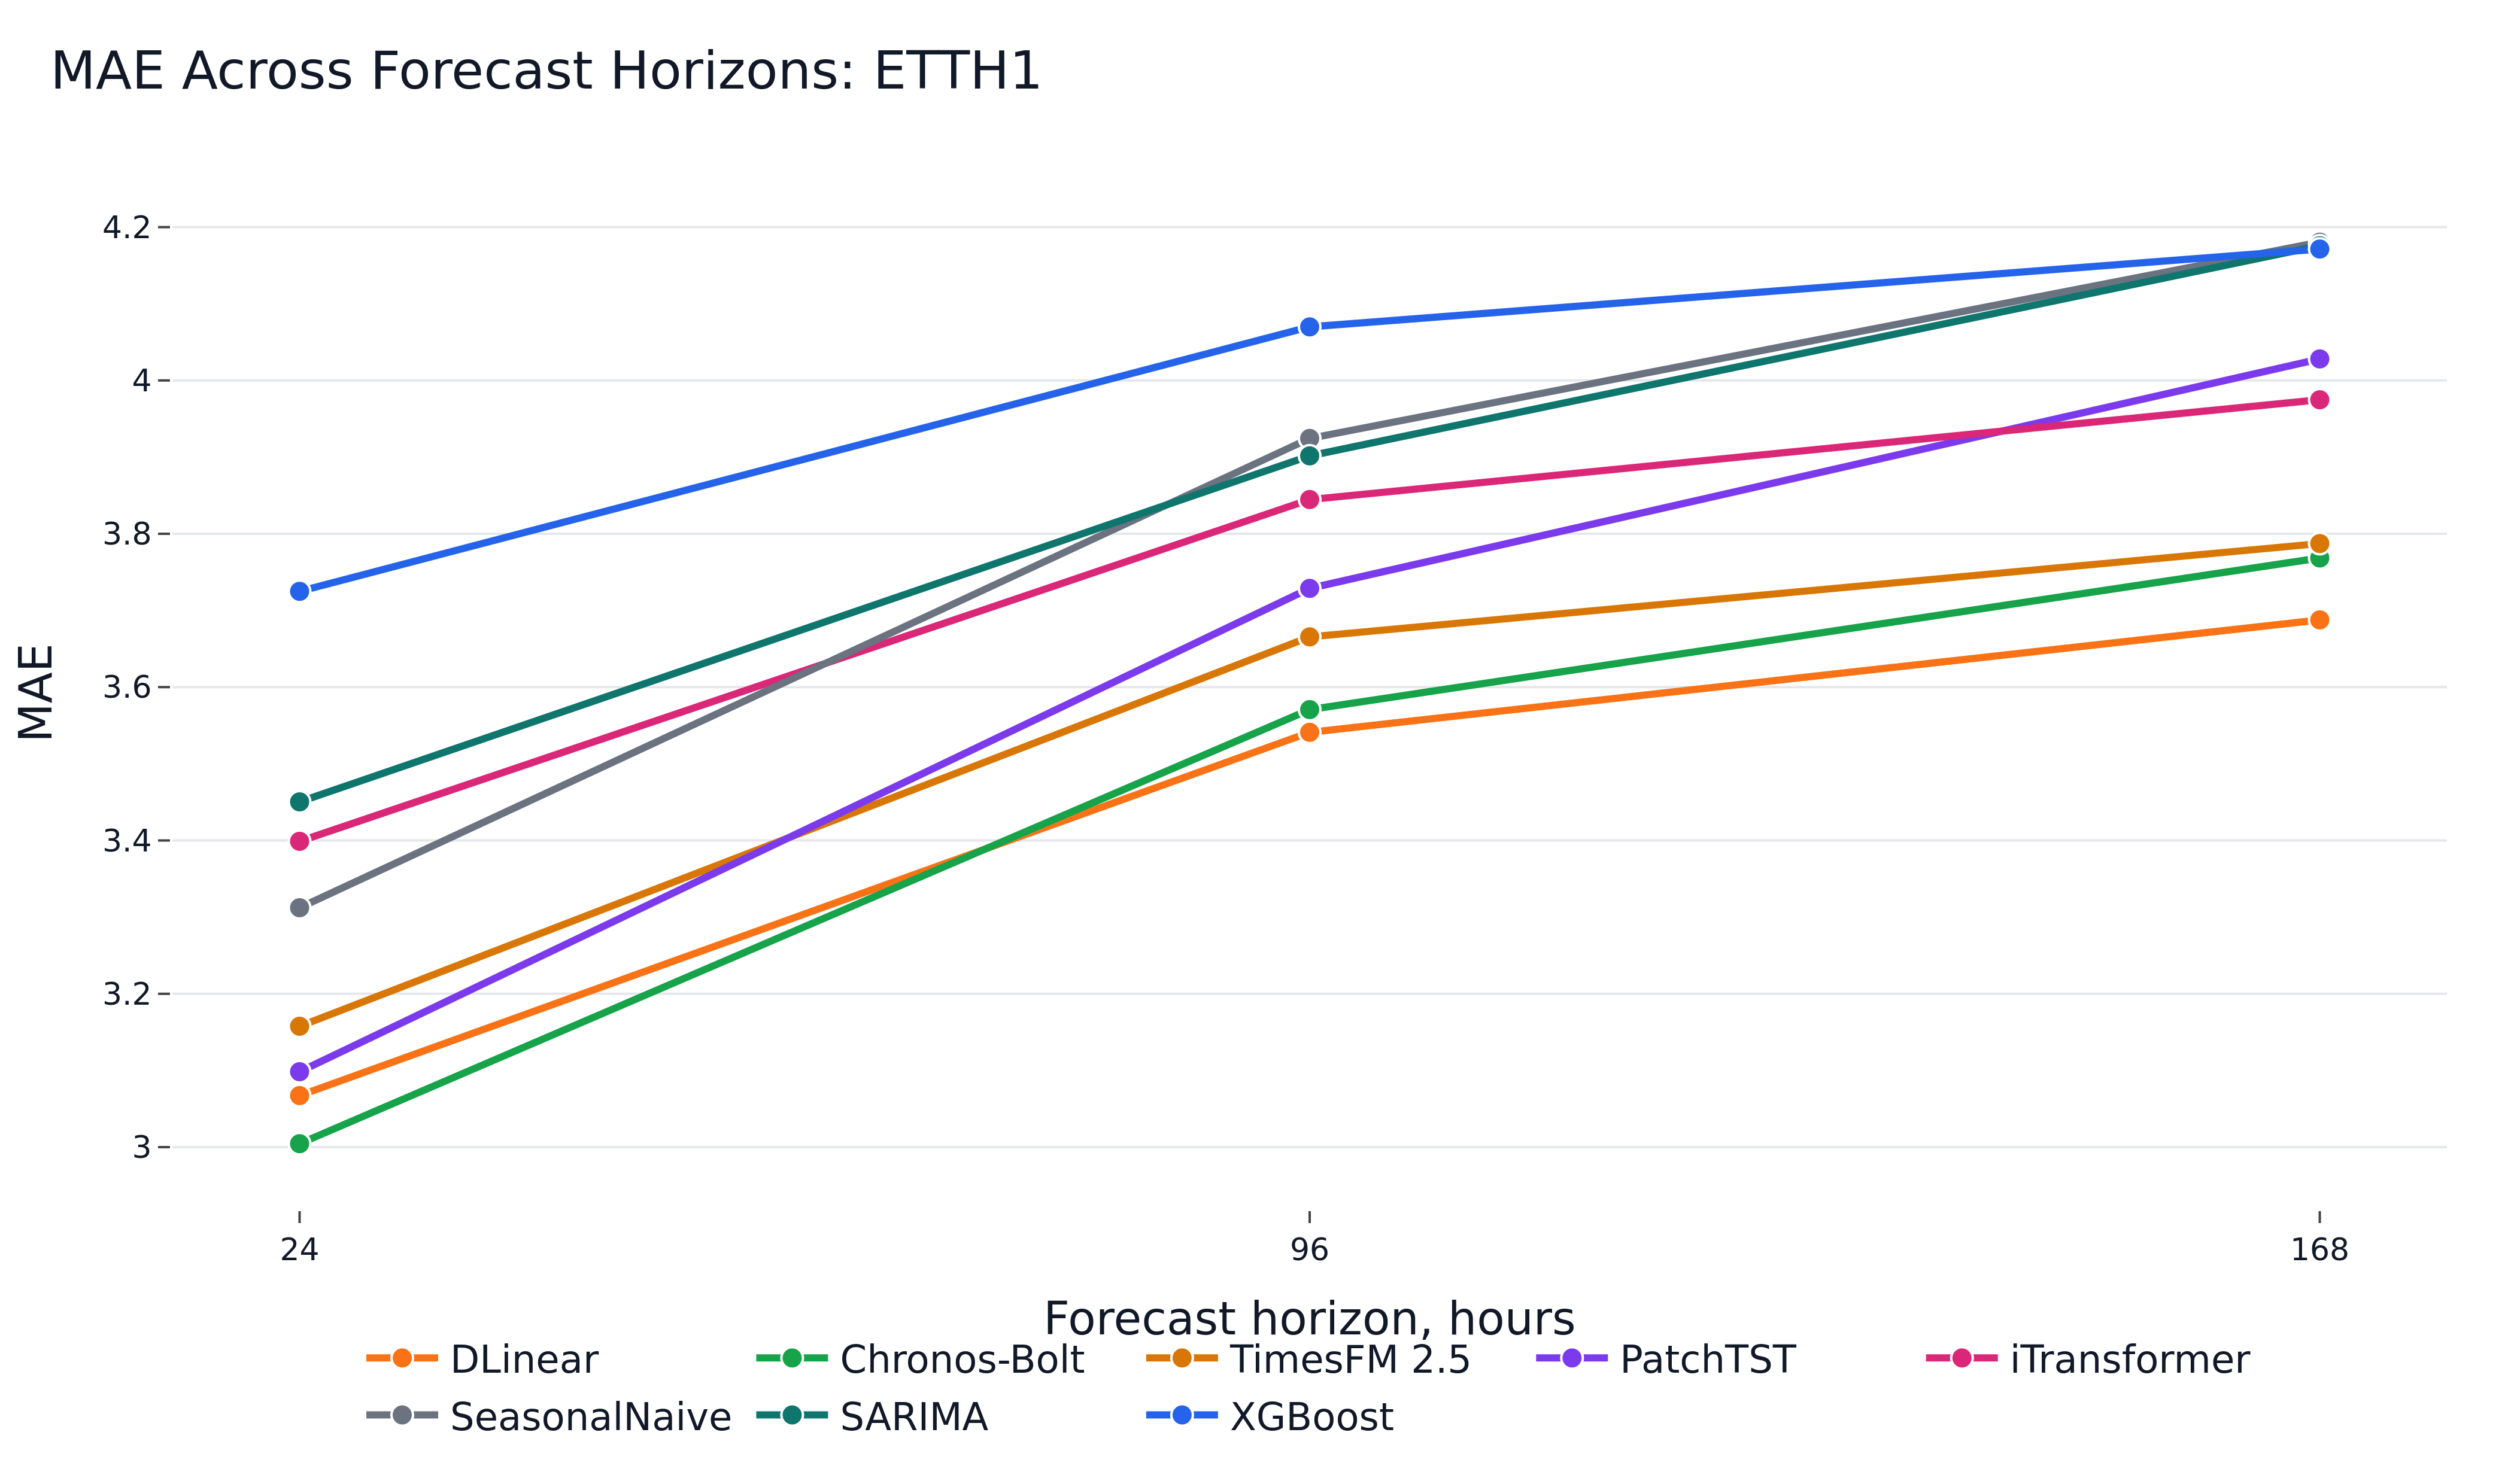
\includegraphics[width=6.6in,height=\textheight,keepaspectratio,alt={Рис. 4. MAE по горизонтам прогноза на ETTh1/HUFL.}]{docx_figures/fig7_etth1_accuracy.png}
\caption{Рис. 4. MAE по горизонтам прогноза на ETTh1/HUFL.}
\end{figure}

\subsection{5.3 Кросс-датасетный
взгляд}\label{ux43aux440ux43eux441ux441-ux434ux430ux442ux430ux441ux435ux442ux43dux44bux439-ux432ux437ux433ux43bux44fux434}

Нормализованная тепловая карта подчёркивает, что лучшее семейство
моделей меняется от датасета и горизонта. На ECL XGBoost и две
фундаментальные модели образуют тесную группу. На ETTh1/HUFL
Chronos-Bolt и DLinear доминируют на разных горизонтах. Сводка по
победителям даёт тот же вывод в более компактной форме.

\begin{figure}
\centering
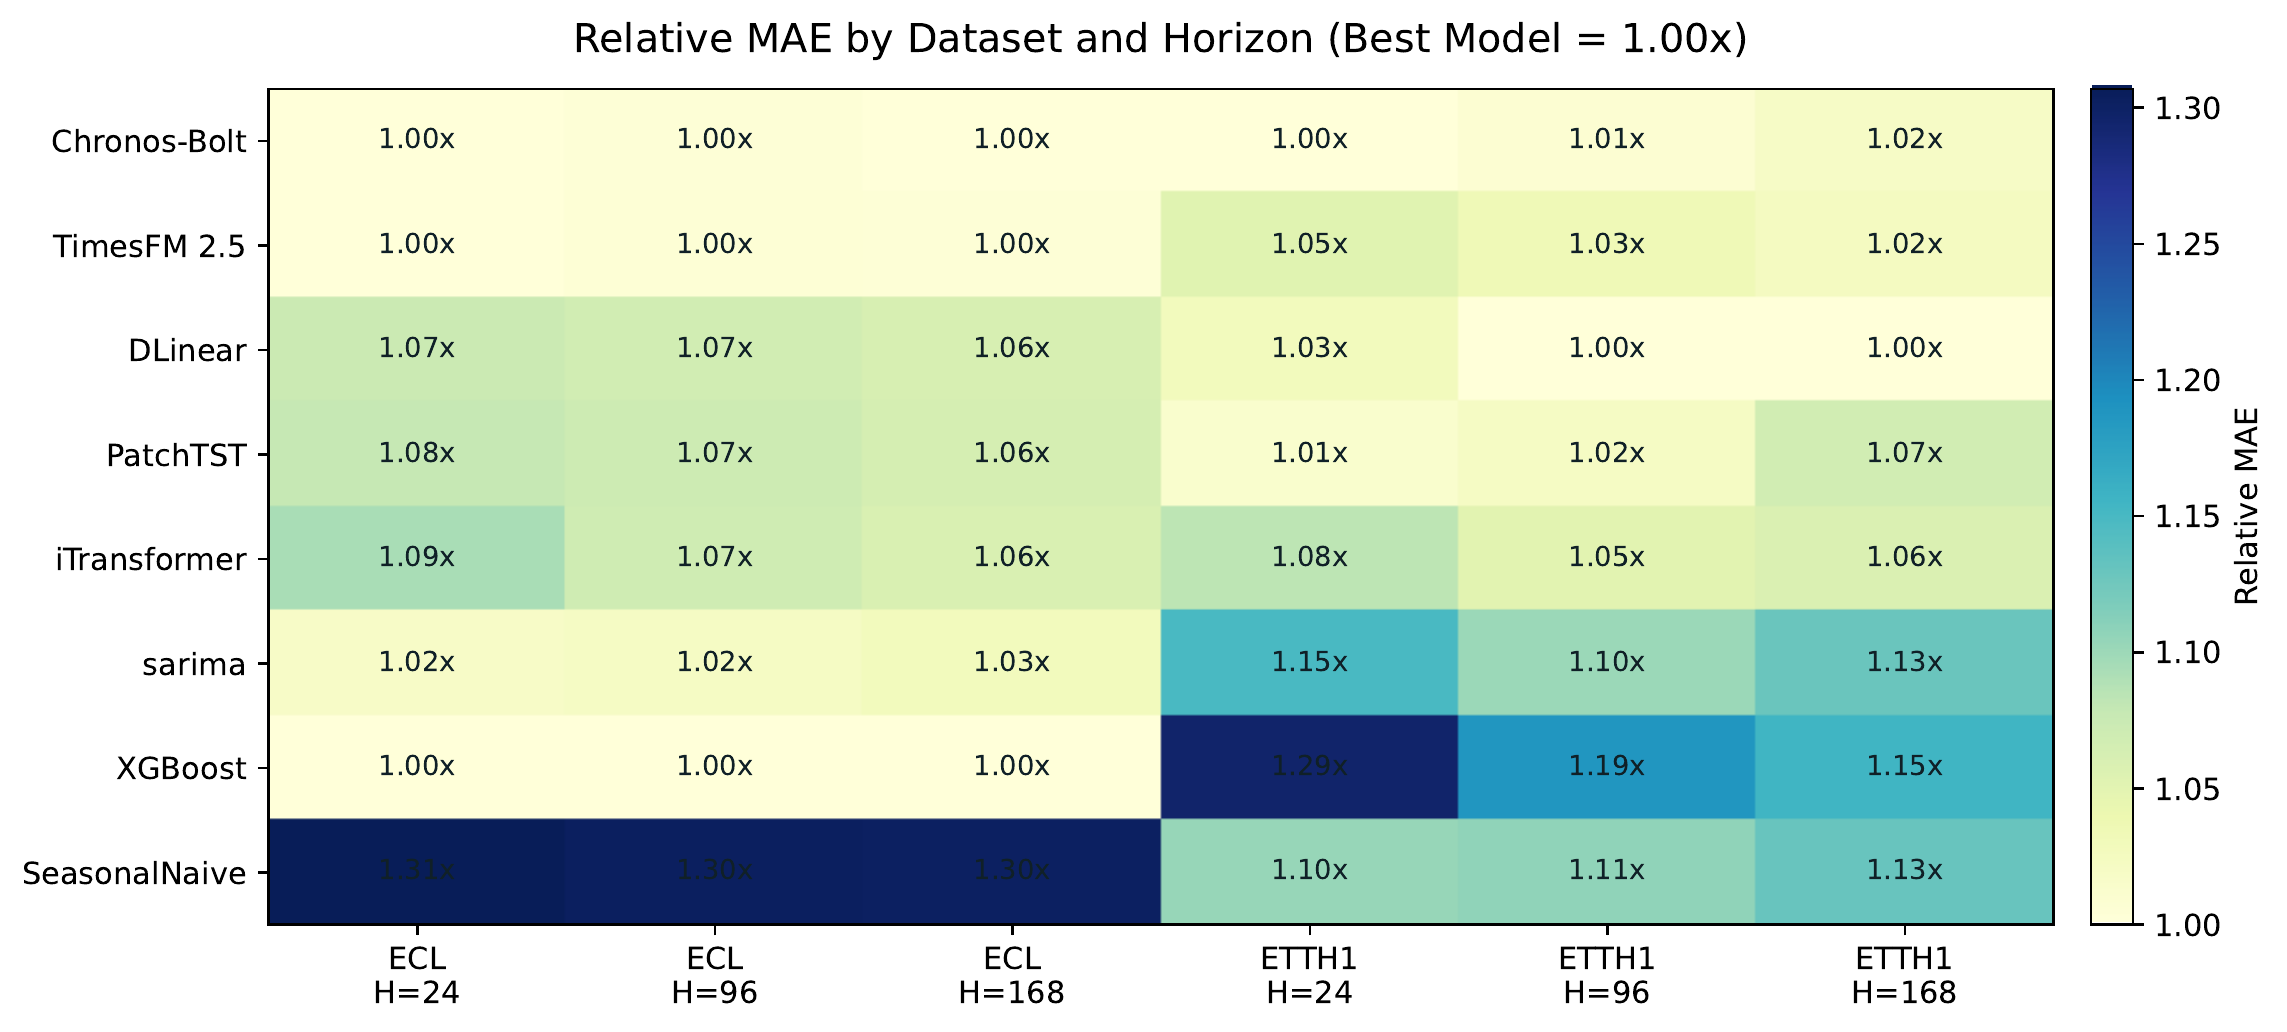
\includegraphics[width=6.6in,height=\textheight,keepaspectratio,alt={Рис. 5. Тепловая карта относительного MAE по датасетам и горизонтам. Значения нормированы внутри пары (датасет, горизонт); лучшая модель равна 1.00.}]{docx_figures/fig3_heatmap.png}
\caption{Рис. 5. Тепловая карта относительного MAE по датасетам и
горизонтам. Значения нормированы внутри пары (датасет, горизонт); лучшая
модель равна 1.00.}
\end{figure}

\begin{figure}
\centering
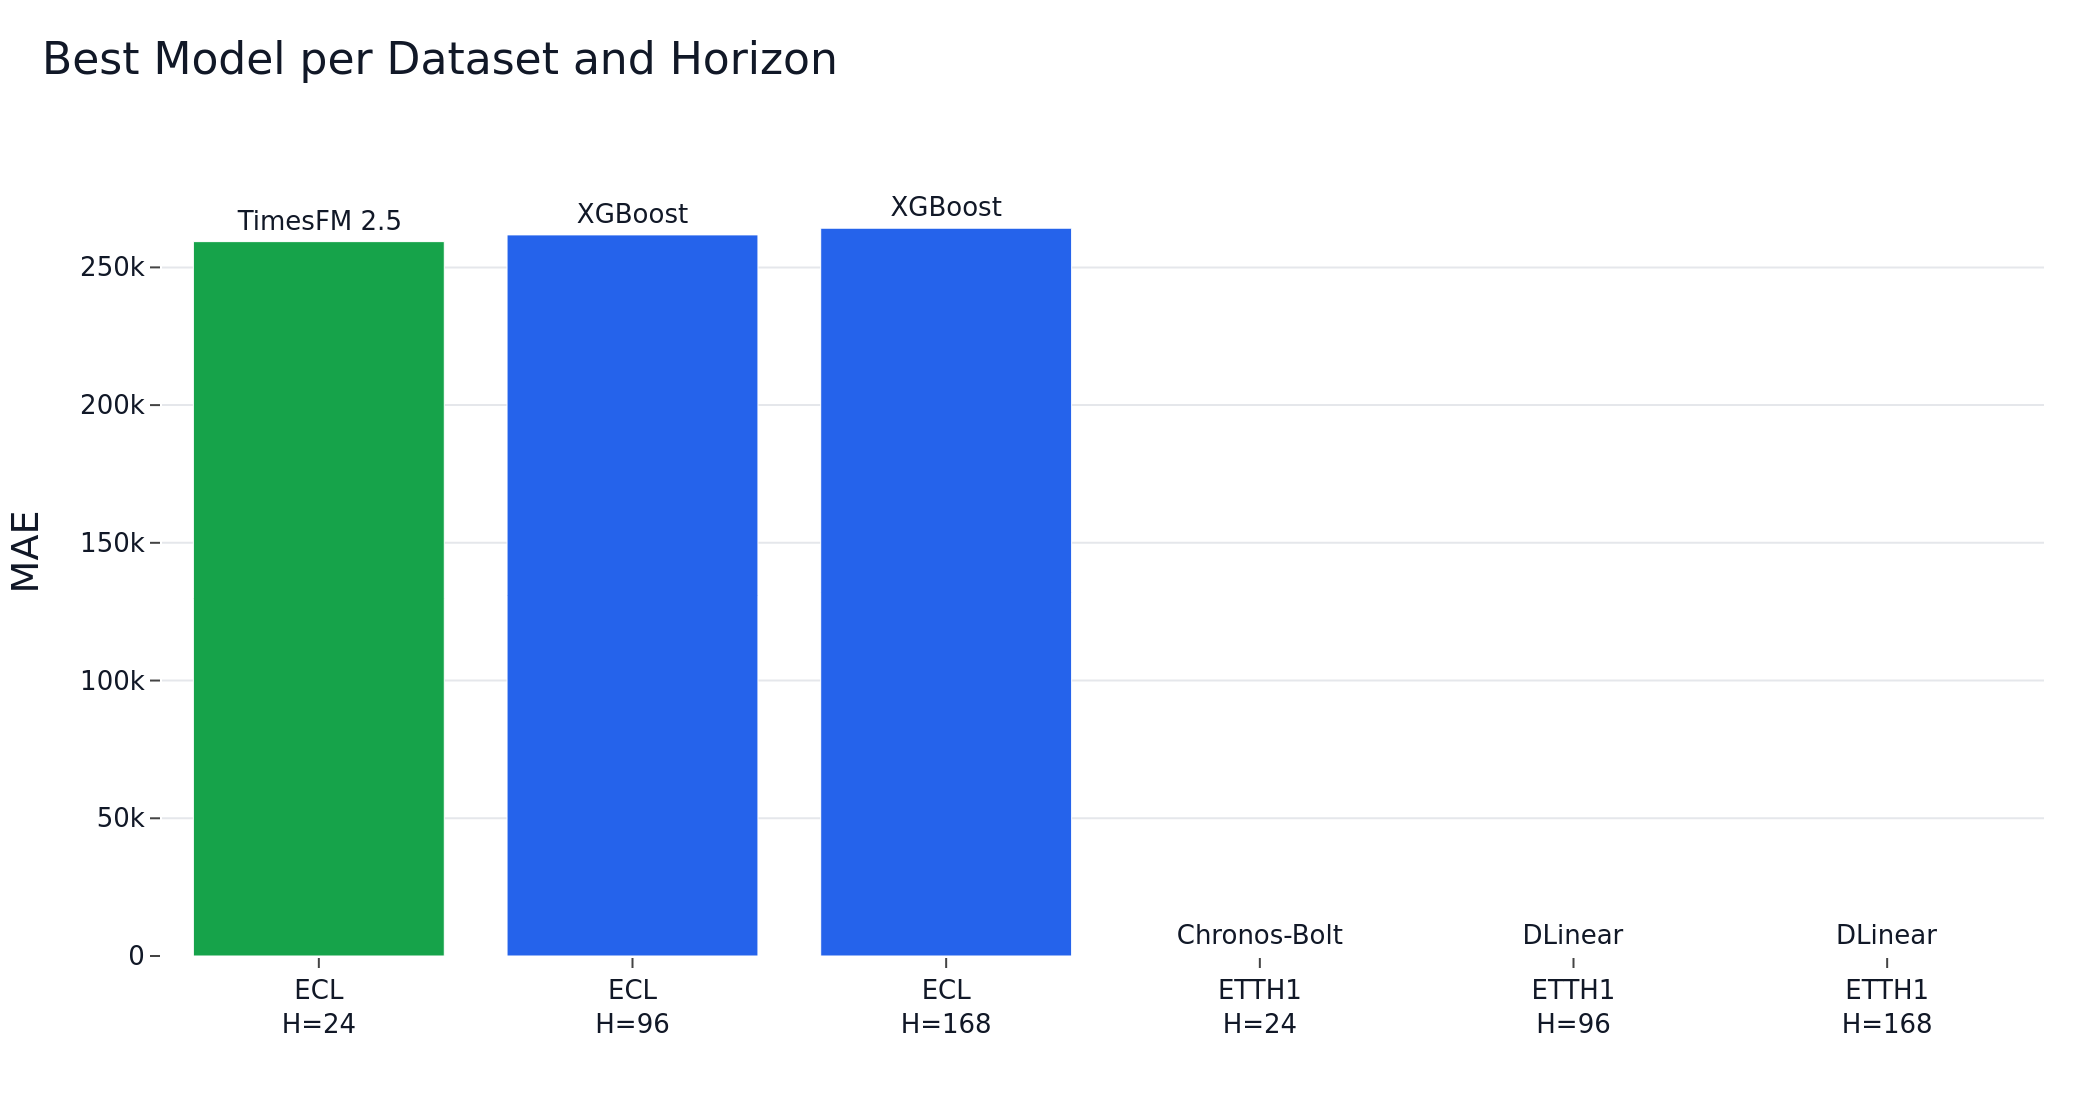
\includegraphics[width=5.8in,height=\textheight,keepaspectratio,alt={Рис. 6. Лучшая модель в каждой паре (датасет, горизонт).}]{docx_figures/fig5_horizon.png}
\caption{Рис. 6. Лучшая модель в каждой паре (датасет, горизонт).}
\end{figure}

\subsection{5.4 Эффективность и статистические
тесты}\label{ux44dux444ux444ux435ux43aux442ux438ux432ux43dux43eux441ux442ux44c-ux438-ux441ux442ux430ux442ux438ux441ux442ux438ux447ux435ux441ux43aux438ux435-ux442ux435ux441ux442ux44b}

Результаты по эффективности отражают компромисс при развёртывании.
SeasonalNaive и SARIMA имеют наименьшую inference latency. XGBoost
остаётся быстрее нейросетевых моделей и TimesFM и не требует GPU.
Chronos-Bolt конкурентен по zero-shot инференсу, тогда как TimesFM имеет
наибольшую latency и потребление GPU-памяти в этой реализации.

{\def\LTcaptype{none} % do not increment counter
\begin{longtable}[]{@{}llrrr@{}}
\toprule\noalign{}
Датасет / H=96 & Модель & MAE & Inference мс/окно & GPU МБ \\
\midrule\noalign{}
\endhead
\bottomrule\noalign{}
\endlastfoot
ECL & XGBoost & 261792.58 & 25.09 & 0.0 \\
ECL & Chronos-Bolt & 262601.94 & 39.64 & 345.8 \\
ECL & TimesFM 2.5 & 262766.32 & 91.99 & 895.6 \\
ETTh1/HUFL & DLinear & 3.55 & 39.29 & 29.8 \\
ETTh1/HUFL & Chronos-Bolt & 3.57 & 36.24 & 345.8 \\
ETTh1/HUFL & XGBoost & 4.21 & 24.47 & 0.0 \\
\end{longtable}
}

\begin{figure}
\centering
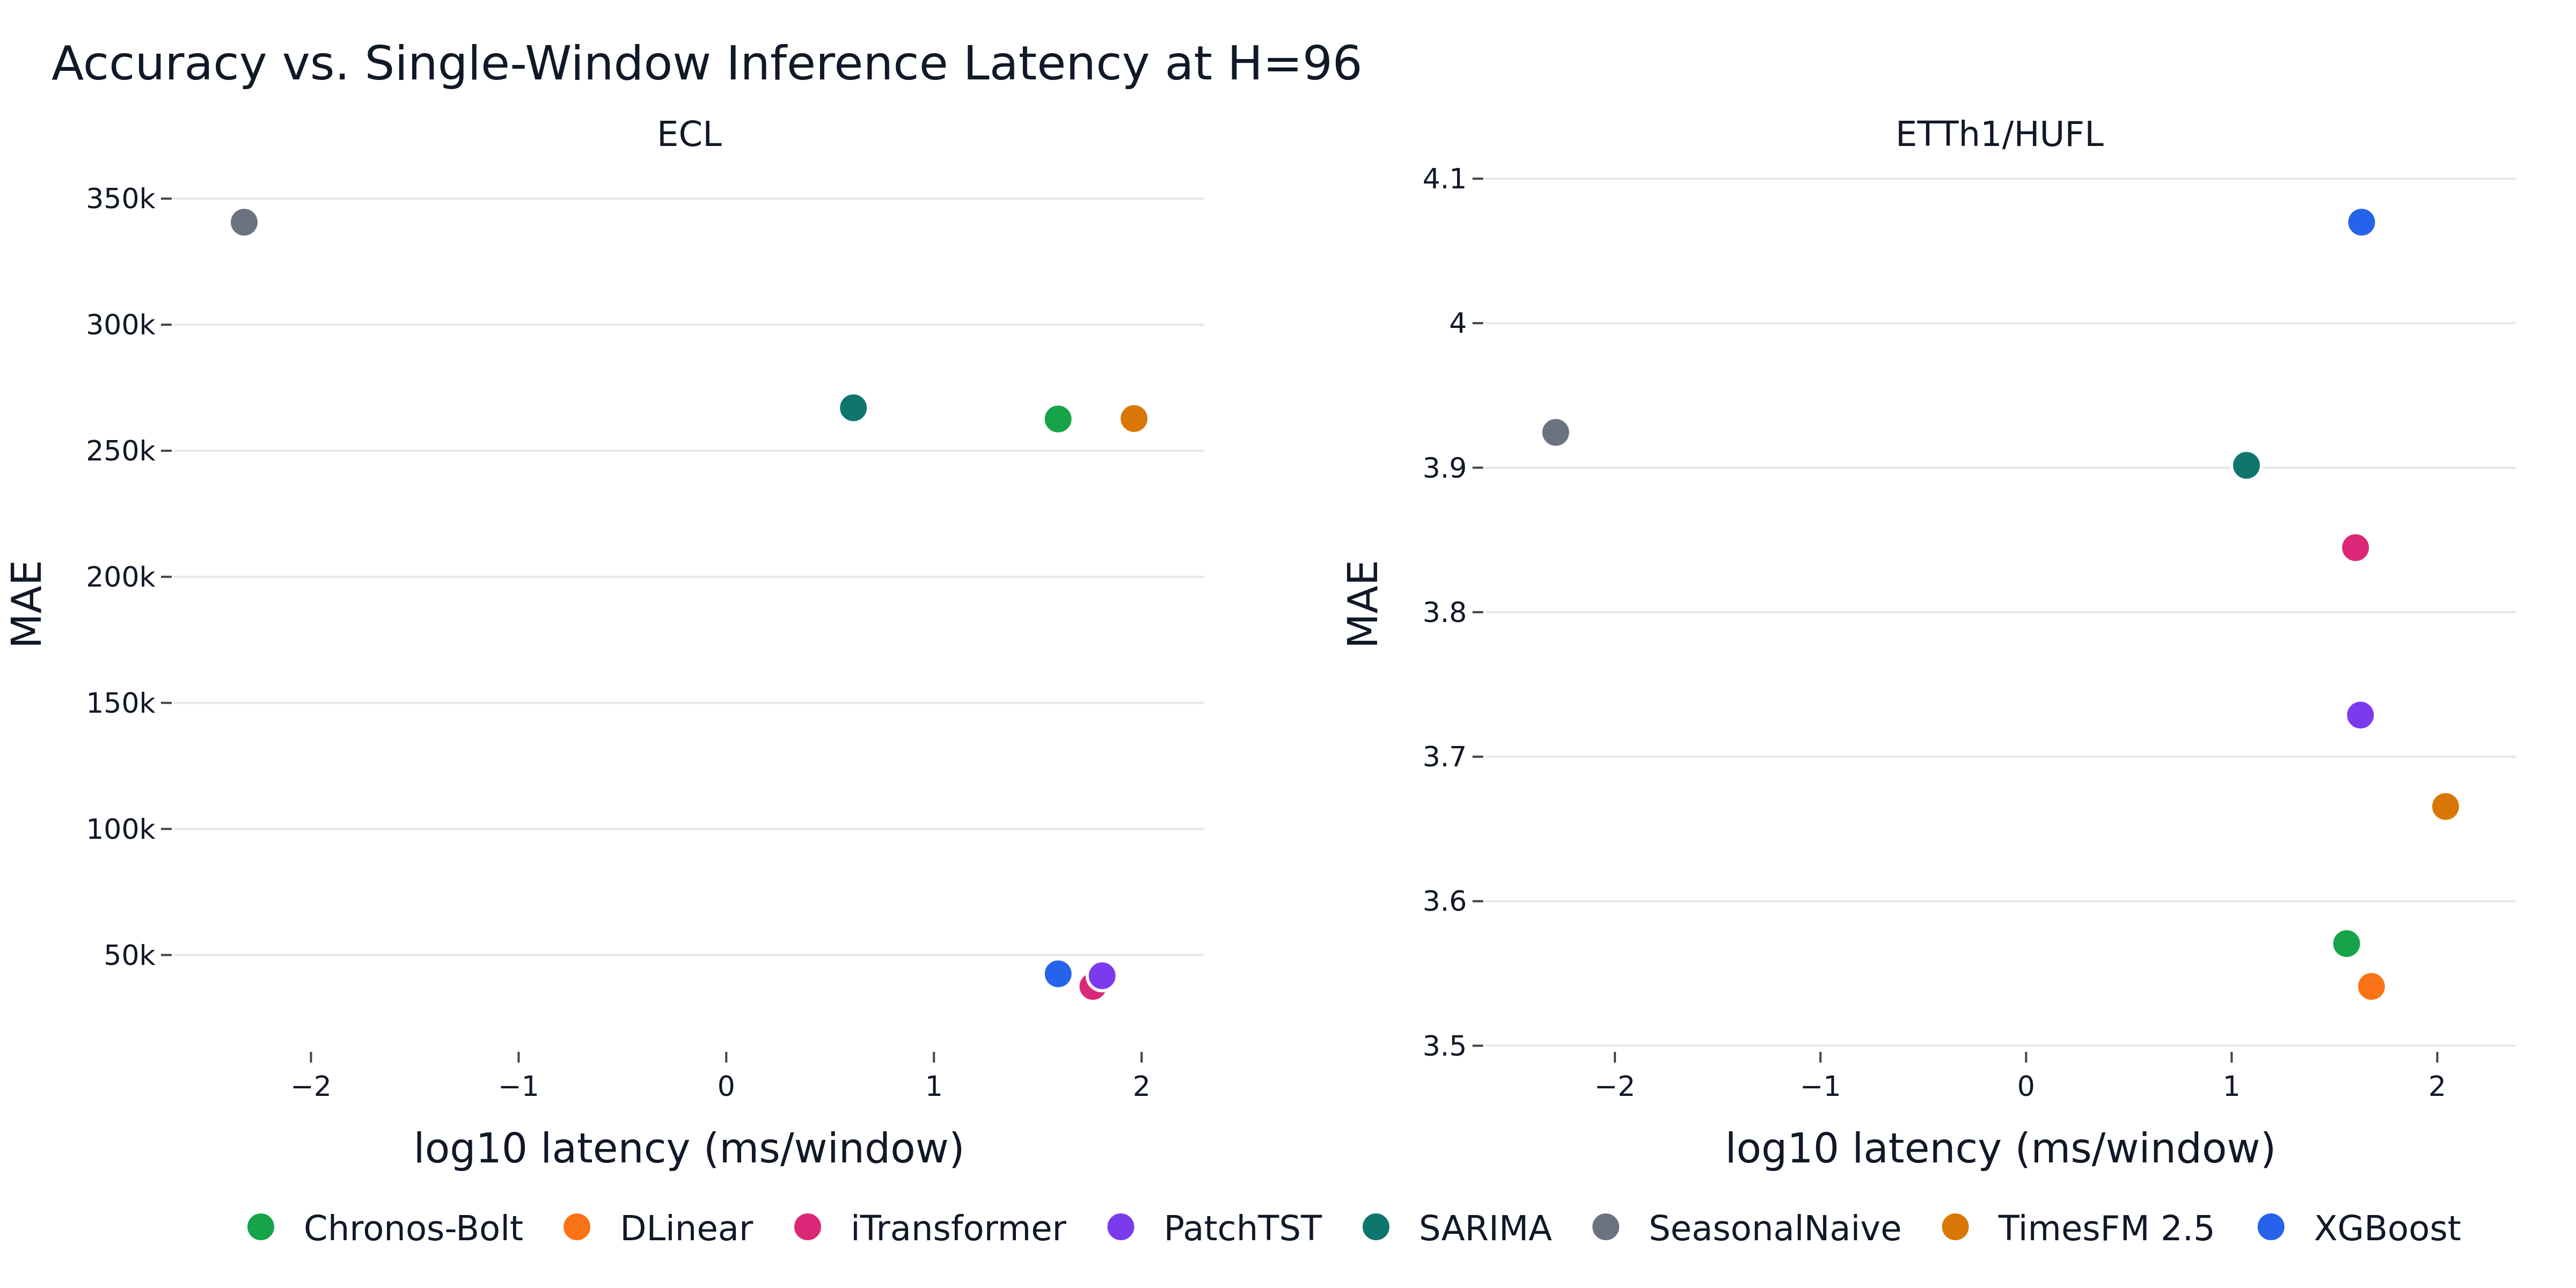
\includegraphics[width=6.6in,height=\textheight,keepaspectratio,alt={Рис. 7. Accuracy--latency при H=96.}]{docx_figures/fig4_pareto.png}
\caption{Рис. 7. Accuracy--latency при H=96.}
\end{figure}

Тесты Дибольда--Мариано подтверждают, что верхние сравнения не сводятся
к небольшим численным различиям в плоском MAE. На ECL результаты при
H=96 и H=168 отдают предпочтение XGBoost над Chronos-Bolt. При H=24
TimesFM и XGBoost практически идентичны в операционном смысле, хотя тест
отвергает гипотезу равной точности. На ETTh1/HUFL тесты подтверждают
Chronos-Bolt при H=24 и DLinear на двух более длинных горизонтах.

{\def\LTcaptype{none} % do not increment counter
\begin{longtable}[]{@{}llrrl@{}}
\toprule\noalign{}
Датасет / Горизонт & Сравнение & Статистика & p-value & Значимо \\
\midrule\noalign{}
\endhead
\bottomrule\noalign{}
\endlastfoot
ECL / H=24 & TimesFM vs XGBoost & 13.45 & \textless0.001 & Да \\
ECL / H=96 & XGBoost vs Chronos-Bolt & -38.15 & \textless0.001 & Да \\
ECL / H=168 & XGBoost vs Chronos-Bolt & -2.88 & 0.004 & Да \\
ETTh1 / H=24 & Chronos-Bolt vs PatchTST & -3.39 & \textless0.001 & Да \\
ETTh1 / H=96 & DLinear vs Chronos-Bolt & -2.48 & 0.013 & Да \\
ETTh1 / H=168 & DLinear vs Chronos-Bolt & -8.81 & \textless0.001 & Да \\
\end{longtable}
}

\section{6.
Обсуждение}\label{ux43eux431ux441ux443ux436ux434ux435ux43dux438ux435}

Результаты показывают, что выбор модели зависит от датасета. На
агрегированной нагрузке ECL инженерия лагов в комбинации с XGBoost
остаётся крайне сильным и недорогим решением. Грид-настроенный SARIMA
также конкурентен и опережает обучаемые нейросетевые архитектуры в этом
сравнении. Фундаментальные модели привлекательны, когда отказ от
обучения на целевом ряду имеет ценность: Chronos-Bolt близок к XGBoost
на ECL и лучший на коротком горизонте ETTh1/HUFL. DLinear --- сильнейшая
обучаемая нейросетевая модель в этом бенчмарке и доминирует на длинных
горизонтах ETTh1/HUFL.

С точки зрения развёртывания модели занимают разные операционные режимы.
XGBoost --- наиболее привлекательный выбор при допустимости стандартного
supervised-пайплайна: точен на ECL, имеет малую single-window latency,
не требует GPU. SARIMA --- конкурентный недорогой запасной вариант без
обучаемых признаков и с миллисекундной инференсной задержкой.
Chronos-Bolt полезен, когда обучение на целевом ряду нежелательно,
например в сценариях cold-start промышленного мониторинга, быстрой
прототипизации или когда данные нельзя объединять для обучения. TimesFM
показывает сильную точечную точность на коротком горизонте ECL, но имеет
существенно более высокую latency в этой реализации.

Результаты трансформеров стоит читать осторожно. PatchTST и iTransformer
--- содержательные архитектуры, однако данный бенчмарк использует
компактную одноцелевую конфигурацию и фиксированный бюджет обучения. Их
относительная слабость здесь не означает общей непригодности
трансформеров для прогноза нагрузки; она лишь показывает, что они не
превосходят более простые методы автоматически в условиях ограниченного
и воспроизводимого протокола.

\section{7.
Ограничения}\label{ux43eux433ux440ux430ux43dux438ux447ux435ux43dux438ux44f}

Основные ограничения связаны с риском контаминации фундаментальных
моделей при претрейне на открытых бенчмарках, ограниченным перебором
гиперпараметров, одноцелевым моделированием и отсутствием закрытых
промышленных данных развёртывания. Скользящий AutoARIMA как базовая
модель пробовался, но полный per-origin grid search оказался непомерно
дорогим в этом протоколе. Частичный запуск сохранён в логах репозитория,
но исключён из основных таблиц сравнения. Грид-настроенный SARIMA в этой
работе --- практическая замена: порядки выбираются на тренировочной
выборке по AICc, и параметры повторно используются для окон прогноза,
давая быстрый и чётко определённый ARIMA-базовый метод.

Chronos-Bolt также выдаёт предупреждение о том, что длины прогноза свыше
64 находятся вне рекомендованного диапазона. Поэтому результаты Chronos
при H=96 и H=168 следует интерпретировать как практический стресс-тест,
а не оптимальное использование модели. Результаты фундаментальных
моделей не следует чрезмерно интерпретировать как гарантированную
zero-shot обобщающую способность на невиданных данных. ECL и ETT ---
открытые бенчмарки, и они могут пересекаться с претрейнинговыми или
оценочными корпусами, использовавшимися при разработке этих моделей.

\section{8.
Заключение}\label{ux437ux430ux43aux43bux44eux447ux435ux43dux438ux435}

Построен и исполнен воспроизводимый пайплайн STLF-бенчмарка на ECL и
ETTh1/HUFL. На ECL XGBoost, Chronos-Bolt и TimesFM операционно близки
друг к другу по горизонтам: TimesFM лучший при H=24, XGBoost --- при
H=96 и H=168. На ETTh1/HUFL Chronos-Bolt лидирует при H=24, PatchTST ---
лучшая обучаемая модель на H=24, DLinear --- при H=96 и H=168. Эти
выводы поддерживают прагматичную рекомендацию: сравнивайте сначала с
сильными простыми базовыми методами, используйте DLinear и PatchTST как
нейросетевые референсы, а фундаментальные модели рассматривайте как
ценный инструмент для cold-start, а не как универсально доминирующую
замену supervised-прогнозированию.

\section*{Литература}\label{ux43bux438ux442ux435ux440ux430ux442ux443ux440ux430}
\addcontentsline{toc}{section}{Литература}

\protect\phantomsection\label{refs}
\begin{CSLReferences}{1}{1}
\bibitem[\citeproctext]{ref-ansari2024chronos}
Ansari, Abdul Fatir, Lorenzo Stella, Caner Turkmen, и др. 2024 г.
{«Chronos: Learning the Language of Time Series»}. \emph{Transactions on
Machine Learning Research}. \url{https://arxiv.org/abs/2403.07815}.

\bibitem[\citeproctext]{ref-chen2016xgboost}
Chen, Tianqi, и Carlos Guestrin. 2016 г. {«XGBoost: A Scalable Tree
Boosting System»}. \emph{Proceedings of the 22nd ACM SIGKDD
International Conference on Knowledge Discovery and Data Mining},
785--94. \url{https://doi.org/10.1145/2939672.2939785}.

\bibitem[\citeproctext]{ref-das2024timesfm}
Das, Abhimanyu, Weihao Kong, Rajat Sen, и Yichen Zhou. 2024 г. {«A
Decoder-Only Foundation Model for Time-Series Forecasting»}.
\emph{International Conference on Machine Learning}.
\url{https://arxiv.org/abs/2310.10688}.

\bibitem[\citeproctext]{ref-hochreiter1997lstm}
Hochreiter, Sepp, и Jürgen Schmidhuber. 1997 г. {«Long Short-Term
Memory»}. \emph{Neural Computation} 9 (8): 1735--80.
\url{https://doi.org/10.1162/neco.1997.9.8.1735}.

\bibitem[\citeproctext]{ref-hyndman2008automatic}
Hyndman, Rob J., и Yeasmin Khandakar. 2008 г. {«Automatic Time Series
Forecasting: The forecast Package for R»}. \emph{Journal of Statistical
Software} 27 (3): 1--22. \url{https://doi.org/10.18637/jss.v027.i03}.

\bibitem[\citeproctext]{ref-liu2024itransformer}
Liu, Yong, Tengge Hu, Haoran Zhang, и др. 2024 г. {«iTransformer:
Inverted Transformers Are Effective for Time Series Forecasting»}.
\emph{International Conference on Learning Representations}.
\url{https://arxiv.org/abs/2310.06625}.

\bibitem[\citeproctext]{ref-nie2023patchtst}
Nie, Yuqi, Nam H. Nguyen, Phanwadee Sinthong, и Jayant Kalagnanam. 2023
г. {«A Time Series is Worth 64 Words: Long-term Forecasting with
Transformers»}. \emph{International Conference on Learning
Representations}. \url{https://arxiv.org/abs/2211.14730}.

\bibitem[\citeproctext]{ref-vaswani2017attention}
Vaswani, Ashish, Noam Shazeer, Niki Parmar, и др. 2017 г. {«Attention Is
All You Need»}. \emph{Advances in Neural Information Processing
Systems}. \url{https://arxiv.org/abs/1706.03762}.

\bibitem[\citeproctext]{ref-wu2023timesnet}
Wu, Haixu, Tengge Hu, Yong Liu, Hang Zhou, Jianmin Wang, и Mingsheng
Long. 2023 г. {«TimesNet: Temporal 2D-Variation Modeling for General
Time Series Analysis»}. \emph{International Conference on Learning
Representations}. \url{https://arxiv.org/abs/2210.02186}.

\bibitem[\citeproctext]{ref-zeng2023dlinear}
Zeng, Ailing, Muxi Chen, Lei Zhang, и Qiang Xu. 2023 г. {«Are
Transformers Effective for Time Series Forecasting?»} \emph{Proceedings
of the AAAI Conference on Artificial Intelligence}.
\url{https://arxiv.org/abs/2205.13504}.

\bibitem[\citeproctext]{ref-zhou2021informer}
Zhou, Haoyi, Shanghang Zhang, Jieqi Peng, и др. 2021 г. {«Informer:
Beyond Efficient Transformer for Long Sequence Time-Series
Forecasting»}. \emph{Proceedings of the AAAI Conference on Artificial
Intelligence}. \url{https://arxiv.org/abs/2012.07436}.

\end{CSLReferences}
